\documentclass[12pt]{article}
\usepackage[utf8]{inputenc}
\usepackage{csquotes, amsmath, amssymb, graphicx, tikz, geometry, multicol}
\usepackage{pdfpages}
\geometry{margin=1in}

\setlength{\parindent}{0in}

\begin{document}

\begin{titlepage}

\begin{center}
    \Huge{Recognizing Quadratic Relations Assignment}
    
    \vspace{1in}
    
    \Large{Simon Wu}
    
    \Large{\today}
    
    \vspace{1in}
    
    \Large{MPM2DE-B}

    
\end{center}

\tableofcontents

\end{titlepage}

\section{Question 1}

\subsection{Part A and B}

\begin{center}
 \begin{tabular}{||c | c | c | c||} 
 \hline
 $x$ & y & 1st Difference & 2nd Difference \\ [0.5ex] 
 \hline\hline
 0 & 0 & N/A & N/A \\ 
 \hline
 1 & 1 & 1 & N/A \\ 
 \hline
 2 & 4 & 3 & 2 \\
 \hline
 3 & 9 & 5 & 2 \\
 \hline
 4 & 16 & 7 & 2 \\
 \hline
 5 & 25 & 9 & 2 \\
 \hline
 6 & 36 & 11 & 2 \\
 \hline
 7 & 49 & 13 & 2 \\
 \hline
 8 & 64 & 15 & 2 \\
 \hline
 9 & 81 & 17 & 2 \\
 \hline
 10 & 100 & 19 & 2 \\
 \hline
\end{tabular}
\end{center}

\subsection{Part C}

We can observe that the first differences are increasing at a constant rate, and that as a result, the second differences are all constant (in this case, $2$). From previous observations of the behaviour of parabolas, we can conclude that this data can represent a parabola.

\subsection{Part D}

I believe that this data can be modelled with the equation:

\[
\boxed{
y = x^2
}
\]

\subsection{Part E and F}

From Figure \ref{fig:q1linear}, it can be seen visually that the linear trendline does not fit the data perfectly. The $R^2$ value corroborates this: in this case, $R^2 = 0.93$, which is not $1$ (a perfect fit).

\subsection{Part G}

From Figure \ref{fig:q1poly2}, it can be seen visually that the polynomial trendline fits the data perfectly. The $R^2$ value of $1$ (indicating a perfect fit) corroborates this.

\subsection{Part H}

From Figure \ref{fig:q1poly3}, it can be seen visually that the polynomial trendline fits the data perfectly. The $R^2$ value of $1$ (indicating a perfect fit) corroborates this.

It can also be observed that the equation of best fit of degree $3$ is actually equivalent to the equation of degree $w$ obtained in Figure \ref{fig:q1poly2}, because the coefficient of the term of degree $3$ is $0$, meaning that the term doesn't actually change anything.

\subsection{Part I}

I believe that my table of values represents a quadratic relation, because the polynomial trendline of degree $2$ fit the data perfectly, as indicated by the $R^2$ value of $1$, and the polynomial trendline of degree $3$ was actually equivalent to the trendline equation of degree $2$.

\subsection{Part J}

The equation displayed for the trendline of best fit in Figure \ref{fig:q1poly2} is $y = 0 + 0x + 1x^2$, while the equation I wrote in part D was $y=x^2$. Obviously, these equations are equivalent.

\subsection{Part K}

The trendline of best fit has a zero at $(0,0)$, and the vertex is also located there.

This vertex and zero indicates that a square will have a side length of $0$ when it has a sidelength of $0$, and that the lowest value (the vertex in this case represents a minimum) of the square's area is given when its side length is $0$, and that it is $0$. This obviously makes sense: $0$ is the smallest area of any shape, given that shapes cannot actually have negative values for their area.

\begin{figure}[p]
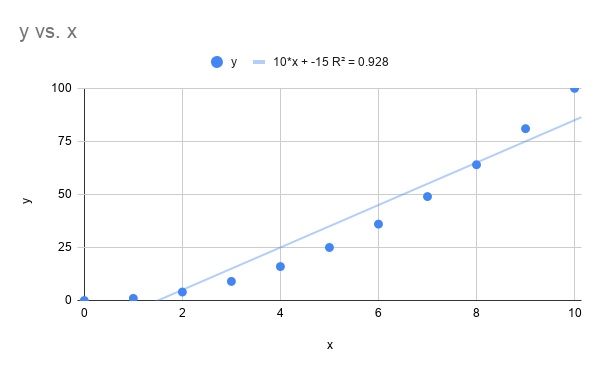
\includegraphics[width=6.5in]{q1graph.png}
\caption{A scatterplot of the data, with a linear trendline and $R^2$ value for this trendline shown. Using a linear regression, it can be shown that the equation of this trendline is $y=10x - 15$.}
\label{fig:q1linear}
\end{figure}

\begin{figure}[p]
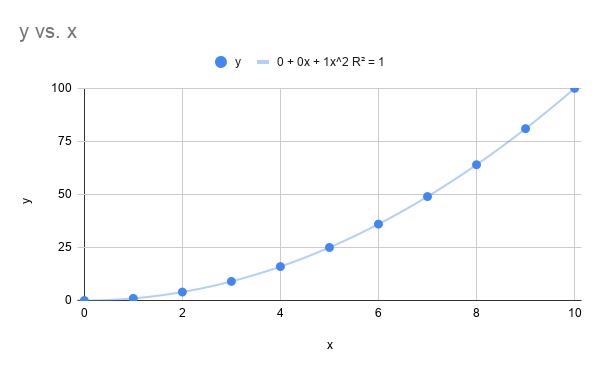
\includegraphics[width=6.5in]{q1graphpoly2.png}
\caption{A scatterplot of the data, with a polynomial trendline of degree $2$ and $R^2$ value for this trendline shown. It can be seen that the equation of this trendline is $y=x^2$.}
\label{fig:q1poly2}
\end{figure}

\begin{figure}[p]
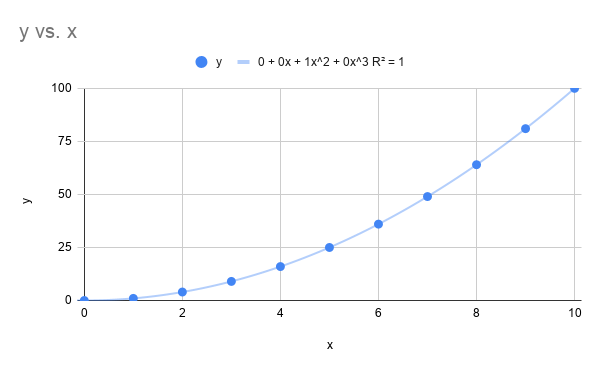
\includegraphics[width=6.5in]{q1graphpoly3.png}
\caption{A scatterplot of the data, with a polynomial trendline of degree $3$ and $R^2$ value for this trendline shown. It can be seen that the equation of this trendline is $y=x^2$: the coefficient of the term of degree $3$ is $0$.}
\label{fig:q1poly3}
\end{figure}


\end{document}